\documentclass{article}
    % General document formatting
    \usepackage[margin=0.7in]{geometry}
    \usepackage[parfill]{parskip}
    \usepackage[utf8]{inputenc}
    \usepackage{amsmath}
    \usepackage{amssymb}
    \usepackage{tikz}
    \usepackage{fancyhdr}
    \usepackage{listings}

\pagestyle{fancy}
\fancyhf{}
\rhead{Edgar Jacob Rivera Rios - A01184125}

\begin{document}
\begin{titlepage}

    \newcommand{\HRule}{\rule{\linewidth}{0.5mm}} % Defines a new command for the horizontal lines, change thickness here

    \center % Center everything on the page

    %----------------------------------------------------------------------------------------
    %	HEADING SECTIONS
    %----------------------------------------------------------------------------------------

    \textsc{\LARGE Tecnológico de Monterrey}\\[1.5cm] % Name of your university/college
    \textsc{\Large Computational intelligence}\\[0.5cm] % Major heading such as course name
    %\textsc{\large Minor Heading}\\[0.5cm] % Minor heading such as course title

    %----------------------------------------------------------------------------------------
    %	TITLE SECTION
    %----------------------------------------------------------------------------------------

    \HRule \\[0.4cm]
    { \huge \bfseries Homework 4}\\[0.4cm] % Title of your document
    \HRule \\[1.5cm]

    %----------------------------------------------------------------------------------------
    %	AUTHOR SECTION
    %----------------------------------------------------------------------------------------

    \begin{minipage}{0.4\textwidth}
    \begin{flushleft} \large
    \emph{Student:}\\
    Jacob \textsc{Rivera} % Your name
    \end{flushleft}
    \end{minipage}
    ~
    \begin{minipage}{0.4\textwidth}
    \begin{flushright} \large
    \emph{Professor:} \\
    Dr. José Carlos \textsc{Bayliss} % Supervisor's Name
    \end{flushright}
    \end{minipage}\\[2cm]

    % If you don't want a supervisor, uncomment the two lines below and remove the section above
    %\Large \emph{Author:}\\
    %John \textsc{Smith}\\[3cm] % Your name

    %----------------------------------------------------------------------------------------
    %	DATE SECTION
    %----------------------------------------------------------------------------------------

    {\large \today}\\[2cm] % Date, change the \today to a set date if you want to be precise

    %----------------------------------------------------------------------------------------
    %	LOGO SECTION
    %----------------------------------------------------------------------------------------

    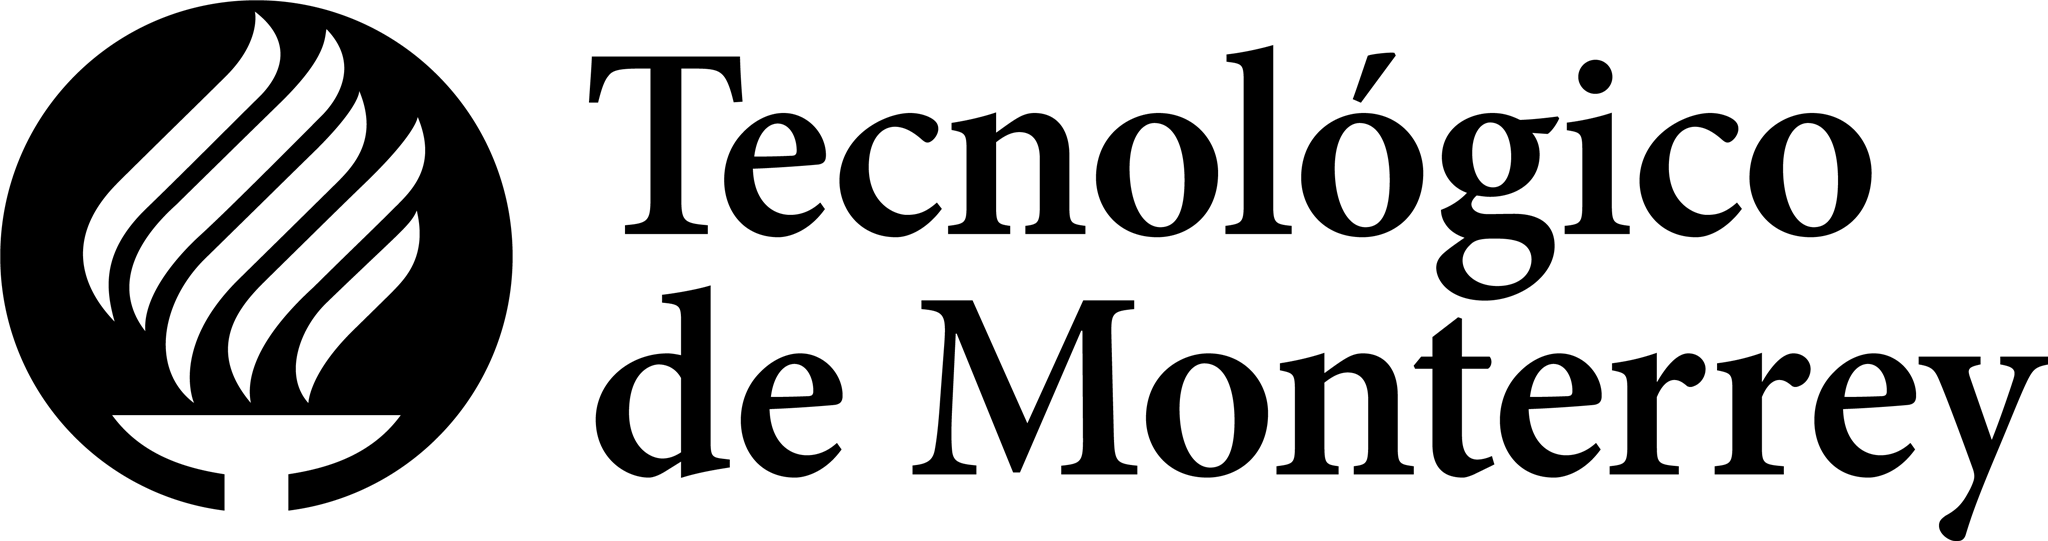
\includegraphics[width=0.4\textwidth,height=\textheight,keepaspectratio]{logo-tec-negro.png} % Include a department/university logo - this will require the graphicx package

    %----------------------------------------------------------------------------------------

    \vfill % Fill the rest of the page with whitespace

\end{titlepage}
\section*{Problems}
\begin{enumerate}
    \item Tournament selection
    \begin{table}[h]
        \centering
        \begin{tabular}{l|l|l}
            & Population & $f$ \\
            \hline
            A & 010111000  & -1 \\
            B & 011101001  & 4 \\
            C & 111000110  & -2 \\
            D & 100001000  & 1 \\
            E & 010101000  & -1
        \end{tabular}
    \end{table}
    \begin{itemize}
        \item How many copies of each chromosome are present in the mating pool?
        \begin{itemize}
            \item A: 0
            \item B: 3
            \item C: 0
            \item D: 2
            \item E: 0
        \end{itemize}
        \item What is the average fitness of the chromosomes in the mating pool? 
        
        2.8

        \item If the tournament size is reduced to one, what is the probability that the chromosome 100001000 appears in the mating pool?
        
        100\%

        \item If the tournament size is increased to five, and both crossover and mutation rate are set to zero, what is the probability that the chromosome 010111000 survives to the next population?
        
        0\%

    \end{itemize}
    
    \item Whole arithmetic crossover
    \begin{align*}
        x=\{ 0.18, 0.75, 0.92, 0.26, 0.44 \}\\
        y=\{ 0.36, 0.77, 0.62, 0.13, 0.51 \}\\
    \end{align*}
    \begin{align*}
        c^{1}_{.5} &= \{ 0.27, .76, .77, .195, .475 \} & c^{2}_{.5} &= \{ 0.27, .76, .77, .195, .475 \}\\
        c^1_{.1} &= \{ 0.342, 0.768, 0.65, 0.143 ,0.503 \} & c^2_{.1} &= \{ 0.198, 0.752, 0.89, 0.247 ,0.447\}\\
    \end{align*}
    
    \pagebreak
    \item Exponential ranking selection 
    \begin{table}[h]
        \centering
        \begin{tabular}{l|l|l}
            & Population & $f$ \\
            \hline
            A & 6661166703  & 5 \\
            B & 3306772232  & 5 \\
            C & 0489794549  & 4 \\
            D & 2660088784  & 4 \\
            E & 3578647359  & 3
        \end{tabular}
    \end{table}


    \item Schemata
    
    
    \item Practical case
    

    \item Analysis
    

\end{enumerate}
\end{document}